\chapter{Principi Fondamentali dell'Interazione}
Un buon design produce un'esperienza piacevole! Ai tecnici non piace molto la parola \textit{esperienza} poiché la considerano troppo soggettiva e poco legata alla tecnologia ed al progresso. Ma se chiediamo ad un ingegnere di descrivere la sua automobile preferita descriverà modello e finiture, dettagli tenici e poi ci narrerà la sensazione che ha provato quando era alla guida: la potenza percepita dall'accelerazione, la maneggevolezza del cambio e dello sterzo, la sensazione di aderenza etc..

L'esperienza è cruciale nell'utilizzo di qualsiasi sistema tecnologico o no che sia. E' grazie all'esperienza che si crea \textbf{la tonalità del ricordo} che conserviamo e associamo agli oggetti con cui abbiamo interagito.

Quando la tecnologia si comporta in maniera inaspettata, gli utenti provano confusione, frustrazione e rabbia: tutte \textbf{emozioni negative}. L'utente che invece riesce a comprendere il funzionamento, e quindi ad utilizzare correttamente un prodotto, proverà una piacevole sensazione di controllo, sarà soddisfatto e persino orgoglio. Tutte queste sensazioni positive saranno associate al prodotto!

\textbf{Cognizione ed emozione sono profondamente legate}: se non si mette l'utente in uno stato mentale positivo e quindi propenso alla sperimentazione e all'interazione, inevitabilmente l'utente compierà più errori perchè avrà un basso interesse per l'oggetto e farà più fatica ad usare l'interfaccia. Più l'utente è arrabbiato e frustrato meno è predisposto ad interagire e quindi imparare come si usa il prodotto e quindi riutilizzarlo in futuro.

Come abbiamo detto nel capitolo precedente, la \textbf{visibilità} o \textbf{discoverability} di un prodotto è il grado di facilità con cui un utente \textbf{scopre cosa può fare, come funziona e che tipo di azioni sono possibili} con il prodotto. 

Tale visibilità si ottiene attraverso il processo di design dell'interazione ed è il risultato dell'applicazione di cinque concetti psicologici fondamentali: 

\begin{itemize}
    \item \textbf{affordance}
    \item \textbf{significanti}
    \item \textbf{mapping} 
    \item \textbf{feedback}
    \item \textbf{vincoli}
\end{itemize}

C'è poi un sesto principio che come vedremo non è legato a degli elementi specifici dell'interfaccia ma piuttosto al concetto generale su cui si va a basare il funzionamento del sistema, \textbf{il modello concettuale del sistema}. Il modello concettuale di un sistema è il cuore dell'interazione e su questo si fonda l'intera esperienza utente.

\section{Affordance}
Il termine affordance, letteralmente \textit{invito}, indica la relazione fra le proprietà di un oggetto o sistema e le proprietà del suo utilizzatore. 

Le affordance non sono quindi proprietà oggettive di un sistema o prodotto ma piuttosto relazioni prodotto-utente che se stabilite abilitano o disabilitano specifiche modalità di interazione fra le parti.

Una sedia appare fatta apposta per sostenere qualcosa quindi \textbf{invita} alla seduta. La maggior parte delle sedie è abbastanza leggera da poter essere sollevata e spostata da una persona possiamo quindi affermare che\\

\textit{una sedia presenta l'affordance per il "sedersi" e per "essere sollevata" da una persona adulta normodotata.}

La sedia non ha infatti la proprietà \textbf{universale} di consentire la seduta a chiunque. Un neonato non riesce a salire su una sedia e non riesce a stare seduto se non ha un sostegno laterale. La sedia non è quindi utilizzabile per sedersi da un neonato quindi per questo utente la sedia NON HA l'affordance del consentire la seduta.

Stessa cosa per la sollevabilità, un bambino di 3 anni può sedersi su una sedia ma non ha abbastanza forza per sollevarla. Quindi, anche in questo caso abbiamo un'affordance che non è disponibile con una categoria di utenti ma lo diventa con altre.

Un'affordance \textbf{non è una proprietà, è una relazione tra un oggetto e utente}, dipende quindi dalle proprietà sia dell'oggetto che dell'utente.

Oltre alle affordance esistono anche le \textbf{anti-affordance}. Un' anti-affordance è una relazione fra oggetto e utente che se stabilita va a negare, vietare alcune proprietà o modi di interazione disponibili fra utente e oggetto.
Un esempio di anti-affordance sono gli "spunzoni" usati come deterrenti per i volatili sui cornicioni, insegne etc. Questo sistema nega all'utente (piccione) di posarsi sul cornicione disabilitando di fatto la altrimenti presente affordance della stazionabilità, supporto, che altrimenti il piccione sarebbe in grado di abilitare e quindi usufruirne.

Le affordance e le anti-affordance per abilitare o disabilitare una particolare modalità di interazione fra oggetto ed utente \textbf{devono essere percepibili, "discoverable"}.

La percepibilità di un affordance non è certo un aspetto ovvio e che può essere dato per scontato. Il vetro, famoso per la sua trasparenza ha "afforda" per la trasmissibilità della luce ma ha un' anti-affordance per l'attraversabilità. Il vetro infatti non consente il passaggio di corpi solidi. Essendo trasparente, questa anti-affordance non è facilmente percepibile dall'utente e quindi l'utente può attuare interazioni non permesse dando origine a problemi di utilizzo (sbattere sulla porta a vetri).

Se uno di questi inviti o impedimenti all'uso non è percepibile c'è bisogno di aumentarne la visibilità e quindi la perceione da parte dell'utente al fine di rendere l'afforndance o anti-affordance percepita e quindi stabilire la corretta modalità di interazione fra utente e oggetto. Per dare visibilità ad un'affordance si usano i \textbf{significanti}.

Spesso nei testi di design si trovano affermazioni tipo: "\textit{E' stata messa un'affordance per...}". Le affordance non si mettono o si tolgono, le affordance sono modalità dell'interazione che nascono da relazioni fra proprietà dell'oggetto e proprietà dell'utente. Per abilitare delle affordance rendendole visibili e quindi palesi all'utente si inseriscono dei significanti che vanno solamente a aumentare la visibilità e compnresione di affordance già presenti.

\section{Significante}
I progettisti hanno dei problemi pratici: hanno bisogno di sapere come rendere comprensibili gli oggetti che creano. Lavorando sulla grafica degli schermi elettronici, dovevano trovare il modo di indicare quali parti potevano essere sfiorate, battute, fatte scivolare in sù, in giù o di lato, azioni che si potevano eseguire con le dita, con lo stilo o con il mouse.

Un significante è quindi \textbf{un modo per indicare dove effettuare un'azione}, data un'affordance che determina quali azioni sono possibili.

\begin{figure}[!h]
	\centering
	\includegraphics[scale = 0.7]{"../immagini/Affordance vs Signifier"}
\end{figure}
\begin{itemize}
	\item \textbf{Affordance}: \textit{cosa si può fare?} \textit{quale azione è possibile compiere?}
	\item \textbf{Signifier}: \textit{dove è possibile fare l'azione?}
\end{itemize}
Molto spesso i significanti \textbf{sono indispensabili} poiché la maggior parte delle affordance sono invisibili. Per fare un esempio basti pensare alle porte scorrevoli: se i cardini non sono visibili, quando vede la maniglia la prima azione che una persona tenta di fare è quella di spingere o di tirare la porta, ma essa non si muoverà, è quindi necessario mettere un significante (e.g. un cartello o una scritta) che indica quale azione è necessaria per aprire la porta.

I significanti posso essere:
\begin{itemize}
	\item \textbf{Voluti o intenzionali}: come un'etichetta, una stringa o un'icona.
	\item \textbf{Accidentali o non intenzionali}: come ad esempio un sentiero tracciato da persone che camminano attraverso un campo o delle persone in fila alla stazione.
\end{itemize}
Nel design \textbf{i significanti sono molto più importanti delle affordances}, perchè comunicano come usare il prodotto o l'interfaccia. Ma come si può associare l'affordance e il significante ad azioni reali? Nella maggior parte dei casi tramite \textbf{convenzioni}. La comprensione di un'affordance percepita è dovuta anche alle convenzioni culturali.

\pagebreak

\begin{figure}[!h]
	\centering
	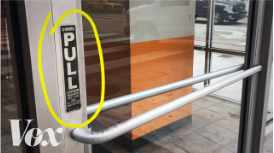
\includegraphics[scale = 0.7]{../immagini/sign.png}
	\caption{La scritta pull è un significante, data l'affordance della porta di essere spinta o tirata.}
\end{figure}
\begin{figure}[!h]
	\centering
	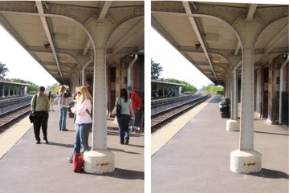
\includegraphics[scale = 0.7]{../immagini/sign1.png}
	\caption{Le persone che aspettano il treno sono un esempio di significante sociale.}
\end{figure}

\section{Mapping}
\textbf{Mapping} è un termine tecnico, ripreso dalla matematica, che indica la relazione fra gli elementi di due insiemi.

Il concetto di \textbf{mapping} è di grande importanza nella progettazione di interfacce, in particolare nel \textbf{posizionamento dei significanti}. La disposizione dei significanti può comunicare di più circa l'interfaccia e circa le sue funzionalità. Infatti se si sfrutta una corrispondenza spaziale fra la collocazione dei comandi e quella dei dispositivi comandati, risulta molto più facile capire come usarli.

Il modo migliore per \textit{fare} mapping è quello \textbf{naturale}, perché è un'attività in cui il cervello umano è molto bravo, i bambini imparano a fare mapping fin dai primi anni di vita. È da tenere presente che il concetto di \textbf{naturale} è ben diverso dal concetto di \textbf{universale}, poiché ci possono essere molti mappings che sembrano naturali ma che in realtà sono specifici a una cerchia di culture.

\begin{figure}[!h]
	\centering
	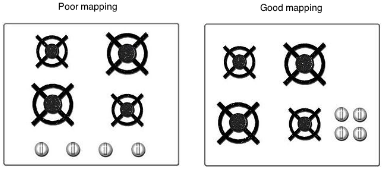
\includegraphics[scale = 0.7]{../immagini/mapping.png}
	\caption{Mapping cattivo e mapping buono.}
\end{figure}

\pagebreak

\section{Feedback}
Il feedback è la comunicazione del risultato di un'azione, è una risposta che l'interfaccia dà all'utente.

Il feedback \textbf{deve essere immediato}, anche un ritardo di un decimo di secondo può essere troppo, se il ritardo è troppo lungo l'utente potrebbe rinunciare all'attività che stava compiendo e passare ad altro o addirittura non riuscire a comprendere l'origine del feedback stesso.

\textbf{Deve essere informativo}, non deve portare con sè troppa informazione, ma deve assolvere al proprio obiettivo, deve far capire che un'azione è in corso o che è stato prodotto il risultato che ci si aspetta. Uno scarso feedback può essere peggio di nessun feedback, perché distrae, crea confusione e di conseguenza frustrazione nell'utente.

Un altro caratteristica importante è \textbf{la semplicità}, un feedback non deve essere pedante: troppi annunci o segnali portano le persone ad ignorarli perdendo anche i feedback cruciali e veramente importanti. Il feedback deve essere \textbf{essenziale} e mantenere l'ambiente calmo e tranquillo.

\section{Modello concettuale}
Un modello concettuale è una descrizione altamente semplificata delle funzionalità di un sistema, non deve essere completa o accurata ma \textbf{utile}. I file, le cartelle e le icone che si vedono sullo schermo del computer aiutano le persone a crearsi un modello concettuale dei dati in memoria o delle applicazioni disponibili. In realtà il computer non contiene fascicoli o cartelle: esse sono solo concettualizzazioni ideate per facilitarne l'uso.

\textbf{I modelli semplificati sono preziosi e utili fintanto che le ipotesi che li supportano sono vere.} Nel cloud storage i file sembrano essere sul dispositivo, ma in molti casi il materiale è in realtà nel cloud. Il modello concettuale veicolato è quello di un archivio disponibile sui dispositivi degli utenti. Questo modello semplificato è utile e basta per il normale utilizzo, ma se il collegamento dei servizi si interrompe, può nascere confusione nell'utente: l'informazione è sempre presente sullo schermo, ma egli non può più salvarla o recuperare altri dati, cosa inspiegabile in relazione al modello concettuale precedentemente veicolato.

Il modello concettuale esprime \textbf{come il designer vuole che l'utente percepisca il prodotto}, sarebbe, in un certo senso, l'ambizione di progettare e comprendere la UX. Una volta che i progettisti hanno pensato e progettato il modello concettuale si implementa l'interfaccia, in modo che il modello concettuale venga veicolato all'utente tramite affordances, significanti e mapping presenti su di essa.

Quando una persona interagisce con il sistema o con il prodotto sviluppa un suo modello mentale. Un \textbf{modello mentale} è un modello concettuale nella mente dell'utente che rappresenta il modo in cui, secondo lui, funzionano le cose. Non solo persone diverse possono avere modelli mentali diversi dello stesso oggetto, ma la stessa persona può avere molteplici modelli, pertinenti ciascuno ad un aspetto diverso del suo funzionamento, e persino contraddittori gli uni con gli altri.

\textbf{Più è grande la differenza tra il modello mentale e quello concettuale, più l'utente farà fatica ad usare il sistema.}

L'ideale è che l'utente apprenda un modello concettuale giusto \textbf{direttamente dal device che utilizza}, senza andare a leggere manuali o istruzioni o, peggio ancora, che gli venga trasmesso da terzi. La comprensione di un dispositivo tramite passaparola porta all'\textbf{effetto del telefono senza fili}: l'interpretazione cambia da persona a persona. Per questo vi è necessità che il modello concettuale trasmesso dal prodotto sia pressoché unico in relazione a quello mentale che l'utente si costruisce. In questo contesto vale l'affermazione \textit{less is more} secondo cui se una feature è difficile da veicolare allora è meglio non implementarla.

\pagebreak

\section{Immagine di Sistema}
Le persone si creano di continuo, attraverso l'esperienza, l'addestramento e l'istruzione, modelli mentali di sé, degli altri, dell'ambiente e degli oggetti con cui esse interagiscono.

Questi modelli servono agli uomini da guida per realizzare i loro scopi e comprendere il mondo in cui vivono.

Come fanno gli uomini a formarsi un modello concettuale adeguato dei dispositivi che utilizzano? Non potendo parlare con il progettista, essi si basano su tutta l'informazione accessibile: l'aspetto dell'apparecchio, cosa hanno imparato dall'uso di oggetti simili in passato, cosa comunicano le pubblicità, i venditori, i pieghevoli illustrativi, il sito web e il libretto di istruzioni.

\textbf{L'insieme di tutta questa informazione è l'immagine di sistema}.

\begin{figure}[!h]
	\centering
	\includegraphics[scale = 0.75]{"../immagini/Immagine di Sistema"}
\end{figure}

Come illustrato nella figura, il progettista e l'utilizzatore finale del prodotto costituiscono i vertici scollegati di un triangolo. Il vertice del triangolo più a destra è occupato dal modello concettuale del progettista, \textbf{cioè dalla sua concezione del prodotto in questione}.

Una volta commercializzato, il prodotto si stacca dal progettista: lo vediamo infatti isolato nel secondo vertice del triangolo.

\textbf{L'immagine di sistema è tutto ciò che si percepisce dalla struttura fisica prodotta, completa di documentazione, istruzioni,significanti e ogni informazione accessibile dal sito web o dal servizio di assistenza clienti}.

Il modello concettuale dell'utente deriva dall'immagine di sistema, mediante l'interazione con il prodotto, mediante letture, ricerche online e manuali. Il progettista si aspetta che il modello concettuale dell'utente coincida col suo, ma, non essendoci comunicazione diretta fra lui e l'utente, tutto il peso della comunicazione grava invece sull'immagine di sistema.

Questo spiega perché la comunicazione è un aspetto importante del buon design. \textbf{ Per quanto sia geniale il prodotto, se la gente non riesce ad usarlo l'accoglienza sarà cattiva}. Tocca al progettista fornire le informazioni adeguate per rendere il prodotto comprensibile ed usabile. Quel che più conta è presentare un modello concettuale capace di guidare l'utente quando le cose non vanno come dovrebbero.

Un buon modello concettuale è la chiave per avere prodotti comprensibili, di facile uso e gradevoli, e una buona comunicazione è importantissima per ottenere buoni modelli concettuali.

\pagebreak

